%% This is file `DEMO-TUDaPub.tex' version 2.09 (2020/03/13),
%% it is part of
%% TUDa-CI -- Corporate Design for TU Darmstadt
%% ----------------------------------------------------------------------------
%%
%%  Copyright (C) 2018--2020 by Marei Peischl <marei@peitex.de>
%%
%% ============================================================================
%% This work may be distributed and/or modified under the
%% conditions of the LaTeX Project Public License, either version 1.3c
%% of this license or (at your option) any later version.
%% The latest version of this license is in
%% http://www.latex-project.org/lppl.txt
%% and version 1.3c or later is part of all distributions of LaTeX
%% version 2008/05/04 or later.
%%
%% This work has the LPPL maintenance status `maintained'.
%%
%% The Current Maintainers of this work are
%%   Marei Peischl <tuda-ci@peitex.de>
%%   Markus Lazanowski <latex@ce.tu-darmstadt.de>
%%
%% The development respository can be found at
%% https://github.com/tudace/tuda_latex_templates
%% Please use the issue tracker for feedback!
%%
%% ============================================================================
%%
% !TeX program = lualatex
%%

\documentclass[
	ngerman,
	accentcolor=1c,% Farbe für Hervorhebungen auf Basis der Deklarationen in den Corporate Design Richtlinien
%	logofile=example-image, %Falls die Logo Dateien nicht vorliegen
	marginpar=false,
	identbarcolor=1c,
	]{tudapub}

\usepackage[english, main=ngerman]{babel}
\usepackage[babel]{csquotes}

\usepackage{biblatex}
\bibliography{DEMO-TUDaBibliography}

%Formatierungen für Beispiele in diesem Dokument. Im Allgemeinen nicht notwendig!
\let\file\texttt
\let\code\texttt
\let\pck\textsf
\let\cls\textsf





%% LOAD CONFIGURATION

% USEPACKAGE
% changed counter for section wise counting
\usepackage{chngcntr}
\usepackage[utf8]{inputenc}
\usepackage[T1]{fontenc}
\usepackage[ngerman]{babel}
\usepackage{graphicx}
\usepackage{subcaption}
\usepackage{listings}
\usepackage{todonotes}
\usepackage[hyphens]{url}
\usepackage{ifthen}
\usepackage{array,multirow,colortbl}

\newboolean{withJava}
\newboolean{doc}
\newboolean{devDoc}
\newboolean{solution}
\newboolean{tasks}
\newboolean{intro}
\newboolean{scoring}

\counterwithin{figure}{section} 
\counterwithin{table}{section} 

\newcommand{\gcenter}[4]{
	\begin{figure}[h]
	\centering 
	\includegraphics[width=#4]{#1}
	\caption{#2}
	\label{fig:#3}
	\end{figure}
}

\newcommand{\easygcenter}[2]{
	\begin{figure}[h]
	\centering 
	\includegraphics[width=#1]{#2}
	\end{figure}
}

\newcommand{\gcenterone}[1]{
	\begin{figure}[h]
	\centering 
	\includegraphics[width=.9\textwidth]{#1}
	\end{figure}
}

\newcommand{\td}[1]{
	\todo[inline]{#1}
	}
	
\newcommand{\sol}{\begingroup
	\catcode`_=12 \docodelst}

\newcommand{\docodelst}[1]{
	\lstinputlisting[caption=\texttt{#1.java}]{\solpath/#1.java}
	\endgroup
}

%makes bold code snippets
\newcommand{\bfcode}[1]{\texttt{\textbf{#1}}}

%fixes enum labels
\renewcommand{\labelenumi}{\theenumi .}
\renewcommand{\labelenumii}{\theenumii )}

%define colors for listings		
\definecolor{javared}{rgb}{0.6,0,0} 			% for strings
\definecolor{javagreen}{rgb}{0.25,0.5,0.35}    	% comments
\definecolor{javapurple}{rgb}{0.5,0,0.35} 		% keywords
\definecolor{javadocblue}{rgb}{0.25,0.35,0.75}  % javadoc

%configure listings for Java Code 
\lstset{
	language=Java,
	breaklines=true,
	postbreak=\mbox{$\hookrightarrow$\space},
	basicstyle=\ttfamily\footnotesize,
	%set colors
	keywordstyle=\color{javapurple}\bfseries,
	stringstyle=\color{javared},
	commentstyle=\color{javagreen},
	morecomment=[s][\color{javadocblue}]{/**}{*/},
	%set line numbering
	numbers=left,
	numberstyle=\tiny\color{black},
	%stepnumber=2, %is uncommented numers every 2nd line
	numbersep=10pt,
	tabsize=4,
	showspaces=false,
	showstringspaces=false
}

%% MANAGE BOOLEANS

% DOCU

\setboolean{withJava}{true}
\setboolean{doc}{true}
\setboolean{devDoc}{false}

% TASKS
\setboolean{tasks}{false}
\setboolean{solution}{false}
\setboolean{intro}{true}
\setboolean{scoring}{false}

%relative path to workshop solutions folder
\newcommand{\solpath}{solutions}

\newcommand{\mySecName}{DUMMY}

\ifthenelse{\boolean{devDoc}}
{\renewcommand{\mySecName}{Abschnitt}}
{\renewcommand{\mySecName}{Aufgabe}}
\ifthenelse{\boolean{doc}}
{\renewcommand{\mySecName}{Abschnitt}}
{\renewcommand{\mySecName}{Aufgabe}}

\makeatletter
\newcommand{\TUD@sectionname@de}{\mySecName}
\makeatother






\begin{document}

%Zusätzliche Metadaten für PDF/A. In diesem Fall notwendig, weil Titel ein Makro enthält.
\Metadata{
	author=NeXT,
	title=Mindroid Template,
	%subject=Basisdokumentation und Template zur Nutzung der tudapub-Dokumentenkasse,
	%date=2019-04-29,
	%keywords=TU Darmstadt \sep Corporate Design \sep LaTeX
}




\title{Space Workshop\newline Dokumentation}
\subtitle{NeXT Generation on Campus}
%\author{Marei Peischl\thanks{pei\TeX{} \TeX{}nical Solutions}\and der \TeX-Löwe}
\date{}
%\titleimage{
%%	%Folgende Box kann selbstverständlich durch ein mit \includegraphics geladenes Bild ersetzt werden.
%\bigskip
%\bigskip
%\bigskip
%\bigskip
%\bigskip
%\bigskip
%\bigskip
%\bigskip
%\bigskip
%\bigskip
%\bigskip
%%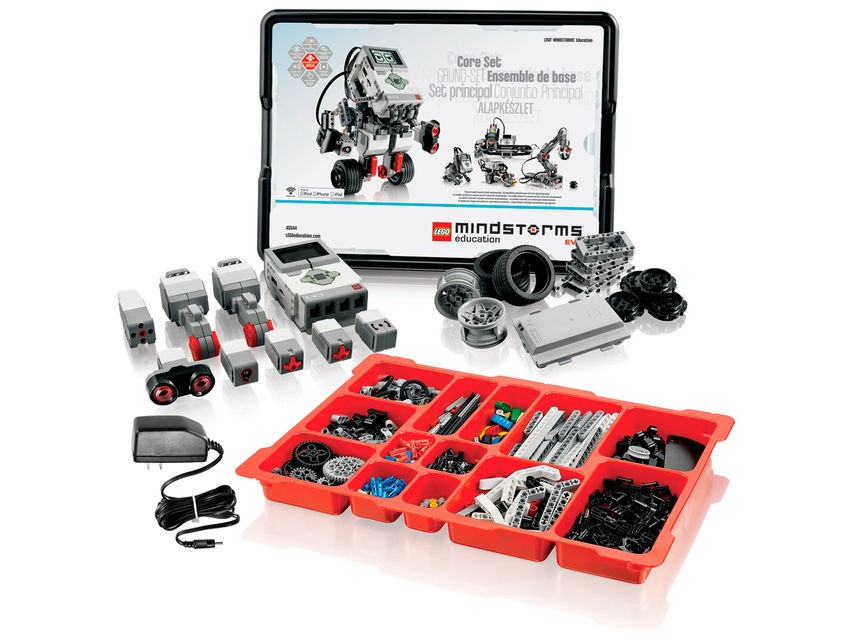
\includegraphics[width=\textwidth]{images/title.jpg}
%	%\color{black!30}\rule{\width}{\height}
%}


%Varianten der Infoboxen
%\addTitleBox{\includegraphics[width=\linewidth]{images/ist_logo.pdf}}
%\addTitleBoxLogo{example-image}
%\addTitleBoxLogo*{\includegraphics[width=.3\linewidth]{example-image}}



%\maketitle


%\newpage


	\titleimage{
	\centering
	%	%Folgende Box kann selbstverständlich durch ein mit \includegraphics geladenes Bild ersetzt werden.
	\bigskip
	\bigskip
	\bigskip
	\bigskip
	\bigskip
	\bigskip
	\bigskip
	\bigskip
	\bigskip
	\bigskip
%	\bigskip	
	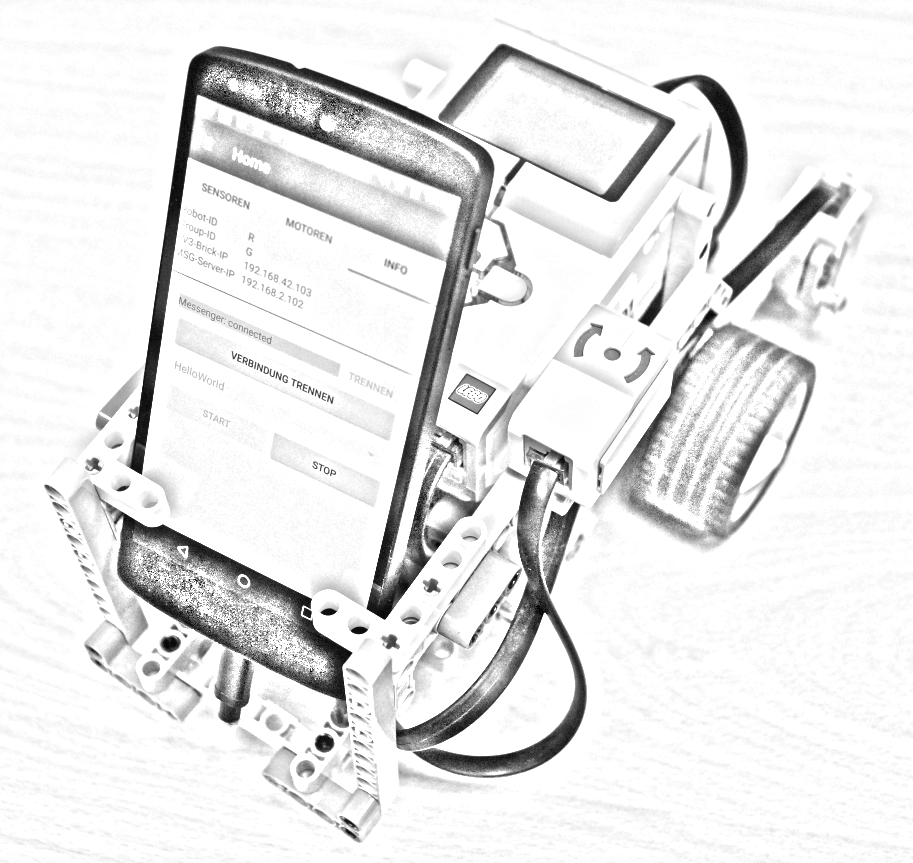
\includegraphics[width=0.8\textwidth]{MindroidTitle.png}
	%\color{black!30}\rule{\width}{\height}
}


%Varianten der Infoboxen
\addTitleBox{\includegraphics[width=\linewidth]{../ist_logo.pdf}}
%\addTitleBoxLogo{example-image}
%\addTitleBoxLogo*{\includegraphics[width=.3\linewidth]{example-image}}
	
	
	
	\newcommand{\titletext}{No Title - No Content}
	
	\ifthenelse{\boolean{doc}}{
		\renewcommand{\titletext}{Dokumentation}
	}{}
	\ifthenelse{\boolean{devDoc}}{
		\renewcommand{\titletext}{Entwickler-Dokumentation}
	}{}
	
	\ifthenelse{\boolean{tasks}}{
		\ifthenelse{\boolean{solution}}{
			\renewcommand{\titletext}{Aufgabenstellung \\mit Lösungen}
		}{
			\renewcommand{\titletext}{Aufgabenstellung}
		}
	}{
		\ifthenelse{\boolean{solution}}{
			\renewcommand{\titletext}{Lösungen}
		}{}
	}


	\pagenumbering{arabic}	
	\title{Mindroid Workshop \\ \titletext}
	\subtitle{NeXT Generation on Campus\newline TU Darmstadt}
%	\subsubtitle{}
	
	\maketitle	
	
	\ifthenelse{\boolean{solution}}{
		\centering	
		\bigskip\bigskip\bigskip\bigskip\bigskip\bigskip\bigskip\bigskip\bigskip	
		{\Huge LÖSUNGEN}
		\newpage
	}{	
%	\bigskip\bigskip\bigskip\bigskip\bigskip
%		\easygcenter{.9\textwidth}{logo/MindroidTitle.png}
%		\newpage
}
	
	
	\ifthenelse{\boolean{doc}}{
			
	
	\section{Einführung}
	In dieser Übersicht werden die Funktionen, die zur Steuerung der Roboter zur Verfügung stehen erklärt.
	Zur Verdeutlichung ein kleines Beispiel:
	
		\begin{table}[htbp]
		\begin{tabular}{|p{0.2\textwidth} p{0.75\textwidth}|}
			\hline
			\textbf{Typ} & \textbf{Methode und Beschreibung} \\ \hline
			void & delay(long milliseconds) \\ 
			&\\
			& Verzögert die Ausführung um die angegebene Zeitspanne (Milisekunden)\\ \hline
		\end{tabular}
		\end{table}
	
	Die Spalte \textit{Typ }gibt an, welchen Typ der Rückgabewert der Funktion hat. \textit{void} bedeutet, dass kein Wert zurück gegeben wird. 
	In der Klammer hinter dem Funktionsnamen wird angegeben, welche Parameter die Funktion erwartet, und von welchem Typ diese sein müssen. In unserem Beispiel bedeutet dies, dass die \textit{delay}-Methode einen Parameter vom Typ \textit{long} (ganzzahliger Wert) erwartet, welcher \textit{milliseconds }genannt wird. 
	Ein möglicher Funktionsaufruf sieht wie folgt aus:
	
	\begin{lstlisting}
	public void run(){	
		delay(1000);
	}
	\end{lstlisting}
	
	Dabei wird die delay-Methode mit 1000 als Parameter aufgerufen. Das bedeutet, die Ausführung wird um $1000ms$ ($= 1s$) verzögert.
	
	
	\subsection{isInterrputed}
	Damit die Ausführung des Programms auch in Schleifen unterbrochen werden kann, sollte jede Schleife die isInterrupted-Methode abfragen. 
	
	Beispiel:
	\begin{lstlisting}
		public void run(){	
			while(!isInterrupted()){
				// Schleifeninhalt
			}
			for(int i=0; i<10 && !isInterrupted(); i++){
				// Schleifeninhalt
			}
		}
	\end{lstlisting}
	
	

	\section{Wichtige Funktionen}
	Hier eine kleine Übersicht über die wichtigsten Funktionen beim Programmieren der Roboter.
	
	\subsection{Fahren}
		\begin{center}\texttt{import org.mindroid.api.ImperativeWorkshopAPI}\end{center}
		
		Mögliche Eingabewerte für den $speed$-Parameter liegen zwischen 0 und 1000.
		Eine maximale Geschwindigkeit von $300$ sollte ausreichen. Niedrigere Geschwindigkeiten schonen den Akku.	
		Die Distanz wird im $distance$-Parameter immer als Kommazahl in Zentimetern (cm) angegeben (z.B.: 20cm werden als $20.0f$ angegeben)
	
		\begin{table}[htbp]
		\begin{tabular}{|p{0.2\textwidth} p{0.75\textwidth}|}
		\hline
		\textbf{Typ} & \textbf{Methode und Beschreibung} \\ \hline
		void & setMotorSpeed(int speed) \\
		& \\
		& Bestimmt die Geschwindigkeit für Fahrmethoden ohne $speed$-Parameter. \\ \hline
		void & forward() \\ 
		void & backward() \\ & \\
		& Fahren mit der von $setMotorSpeed(...)$ gesetzten Geschwindigkeit. \\ \hline
		void & driveDistanceForward(float distance) \\
		void & driveDistanceBackward(float distance) \\ & \\
		& Fahren mit der von $setMotorSpeed(...)$ gesetzten Geschwindigkeit\\ 
		& Die Distanz muss in Zentimetern angegeben werden. \\ \hline
		
		void & forward(int speed) \\ 
		void & backward(int speed)  \\ 
		void & driveDistanceForward(float distance, int speed) \\ 
		void & driveDistanceBackward(float distance, int speed) \\ 		
		& \\
		& Wie oben, nur dass der $speed$-Parameter die von $setMotorSpeed()$ gesetzte Geschwindigkeit überschreibt. Nach Beendigung des Aufrufs, wird wieder die vorher gesetzte Geschwindigkeit genutzt.\\ \hline

		void & turnLeft(int degrees) \\ 
		void & turnRight(int degrees) \\ 
		void & turnLeft(int degrees, int speed) \\ 
		void & turnRight(int degrees, int speed) \\ 
		& \\
		& Dreht den Roboter um den im $degrees$-Parameter bestimmten Wert. \\
		& Der $Speed$-Parameter verhält sich wie bei den anderen Methoden. \\ \hline
		
		void & stop() \\ 
		& \\
		& Stoppt sofort alle Motoren.	\\ \hline
		\end{tabular}
		\end{table}
		
		\newpage
	\subsection{Sensoren}
			\begin{center}\texttt{import org.mindroid.api.ImperativeWorkshopAPI}\end{center}
		\begin{table}[htbp]
		\begin{tabular}{|p{0.2\textwidth} p{0.75\textwidth}|}
		\hline
		\textbf{Typ} & \textbf{Methode und Beschreibung} \\ \hline
		float & getAngle() \\ 
		&\\
		& Liefert den Winkel des Gyrosensors in Grad\\ \hline
		float & getDistance() \\ 
		&\\
		& Liefert die vom Ultraschallsensor gemessene Distanz in Zentimetern\\ \hline		
		Colors & getLeftColor() \\ 
		Colors & getRightColor() \\
		&\\
		& Liefert den Wert des Linken/Rechten Farbsensors\\ 
		& Farbwerte: Colors.BLACK, Colors.BLUE, Colors.BROWN, Colors.GREEN, \\ &Colors.RED, Colors.WHITE, Colors.YELLOW, Colors.NONE\\ \hline
		\end{tabular}
		\end{table}

	\subsection{Kommunikation}
				\begin{center}\texttt{import org.mindroid.api.ImperativeWorkshopAPI}\end{center}
		\begin{table}[htbp]
		\begin{tabular}{|p{0.2\textwidth} p{0.75\textwidth}|}
		\hline
		\textbf{Typ} & \textbf{Methode und Beschreibung} \\ \hline
		boolean & hasMessage() \\ 
				&\\
		& Prüft ob Nachricht vorhanden ist \\ \hline
		MindroidMessage & getNextMessage() \\ 
				&\\
		& Ruft nächste Nachricht ab \\ \hline		
		void & sendBroadcastMessage(String message) \\ 
				&\\
		& Sendet eine Nachricht an alle Roboter \\ \hline
		String & getRobotID() \\ 
				&\\
		& Gibt den Namen des Roboters zurück. \\ \hline
		void & sendLogMessage(String logmessage) \\ 
				&\\
		& Sendet eine Nachricht an den Message Server \\ \hline
		void & sendMessage(String destination, String message) \\ 
				&\\
		& Sendet eine Nachricht an den $destination$-Roboter \\ \hline
		\end{tabular}
		\end{table}
		
		Um eine Nachricht zu empfangen, muss zuerst mit $hasMessage()$ überprüft werden ob eine Nachricht vorhanden ist. Liefert $hasMessage()$ true zurück, kann mit $getNextMessage()$ eine Nachricht abgerufen werden. Das Beispiel in Listing \ref{lst:msg} zeigt wie das geht.
		
		\begin{lstlisting}[captionpos=b, caption=Beispiel zum Abrufen einer Nachricht, label=lst:msg]
		if (hasMessage()){
          String msg = getNextMessage().getContent();
        }
		\end{lstlisting}
		
		$broadcastMessage(...)$ schickt eine Nachricht an alle mit dem selben Message-Server verbundenen Roboter.
		
		\subsection{MindroidMessage}

			Um die von $getNextMessage()$ zurückgegebene Nachricht verarbeiten zu können, muss ein zusätzlicher import hinzugefügt werden.
						\begin{center}import org.mindroid.common.messages.server.MindroidMessage;\end{center}
		
			\begin{table}[htbp]
				\begin{tabular}{|p{0.2\textwidth} p{0.75\textwidth}|}
					\hline
					\textbf{Typ} & \textbf{Methode und Beschreibung} \\ \hline
					String & getContent() \\ 
							&\\
					& Liefert den Inhalt der Nachricht zurück\\ \hline
					RobotID & getDestination() \\ 
					RobotID & getSource() \\ 
							&\\
					& Liefert die Quelle/das Ziel der Nachricht an\\ \hline		
				\end{tabular}
			\end{table}
		
	%\newpage
	\subsection{Brick}
	\subsubsection{Display}
		\begin{table}[htbp]
		\begin{tabular}{|p{0.2\textwidth} p{0.75\textwidth}|}
		\hline
		\textbf{Typ} & \textbf{Methode und Beschreibung} \\ \hline
		void & clearDisplay() \\ 
		&\\
		& Löscht den Aktuellen Inhalt des Displays \\ \hline
		void & drawString(String text)\\			
		void & drawString(String text, int row)\\
		&\\
		& Schreibt den im $text$-Parameter gegebenen Text auf das Display.\\
		& Der Parameter $row$ bestimmt die zu beschreibende Zeile. \\
		& Wird der Parameter $row$ weggelassen, wir in die Mittlere Zeile geschrieben. \\
		\hline

		\end{tabular}
		\end{table}
		\gcenter{img/ev3_display}{Koordinaten der Pixel des Displays des EV3\protect\footnotemark\ }{display}{.5\textwidth}
		
\footnotetext{ \url{https://services.informatik.hs-mannheim.de/~ihme/lectures/LEGO\_Files/01\_Anfaenger\_Graphisch\_EV3\_BadenBaden.pdf}		}

	\newpage
	\subsubsection{Buttons}
							\begin{center}import org.mindroid.impl.brick.Button;\end{center}
		\begin{table}[htbp]
		\begin{tabular}{|p{0.2\textwidth} p{0.75\textwidth}|}
		\hline
		\textbf{Typ} & \textbf{Methode und Beschreibung} \\ \hline
		boolean & isDownButtonClicked() \\ 
		boolean & isEnterButtonClicked() \\ 
		boolean & isLeftButtonClicked() \\ 
		boolean & isRightButtonClicked() \\ 
		boolean & isUpButtonClicked() \\ \hline
		\end{tabular}
		\end{table}

		Die Funktionen liefern $true$ wenn der entsprechende Button gedrückt wurde. Die Benennung der Buttons kannst du Abbildung \ref{fig:buttons} auf Seite \pageref{fig:buttons} entnehmen

		%\newpage
	\subsubsection{Sound}
		\begin{table}[htbp]
		\begin{tabular}{|p{0.2\textwidth} p{0.75\textwidth}|}
		\hline
		\textbf{Typ} & \textbf{Methode und Beschreibung} \\ \hline
		void & setSoundVolume(int volume) \\ 
		void & playBeepSequenceDown() \\ 
		void & playBeepSequenceUp() \\ 
		void & playBuzzSound() \\ 
		void & playDoubleBeep() \\ 
		void & playSingleBeep() \\ \hline
		\end{tabular}
		\end{table}
		
		Der Parameter $volume$ nimmt Werte von 0 bis 10 entgegen.
		
	\newpage
	\subsubsection{LED}		
		\begin{table}[htbp]
		\begin{tabular}{|p{0.2\textwidth} p{0.75\textwidth}|}
		\hline
		\textbf{Typ} & \textbf{Methode und Beschreibung} \\ \hline
		void & setLED(int mode) \\ 
		&\\
		& Lässt die LED des EV3 im angegebenen Modus leuchten\\
		& Der Parameter $mode$ kann entweder als Ganzzahl von 0 bis 9 oder als Konstante angegeben werden. \\
		& Siehe Tabelle \ref{tab:led}\\
		\hline
		
		\end{tabular}
		\end{table}
		
		
		
		\begin{table}[htbp]
		\caption{Funktion der einzelnen Modi der LED}
		\begin{center}
		\begin{tabular}{r|l|l|l}
		
		\multicolumn{2}{c|}{\textbf{Modus (Parameter $mode$)}}   & \textbf{Farbe} & \textbf{Intervall} \\ 
		\multicolumn{1}{l|}{Wert} & Konstante &  &  \\ \hline
		0 & LED\_OFF & Aus & Aus \\ 
		1 & LED\_GREEN\_ON & Grün & Dauer \\ 
		2 & LED\_GREEN\_BLINKING & Grün & Blinken \\ 
		3 & LED\_GREEN\_FAST\_BLINKING & Grün & Schnell Blinken \\ 
		4 & LED\_YELLOW\_ON & Gelb & Dauer \\ 
		5 & LED\_YELLOW\_BLINKING & Gelb & Blinken \\ 
		6 & LED\_YELLOW\_FAST\_BLINKING & Gelb & Schnell Blinken \\ 
		7 & LED\_RED\_ON & Rot & Dauer \\ 
		8 & LED\_RED\_BLINKING & Rot & Blinken \\ 
		9 & LED\_RED\_FAST\_BLINKING & Rot & Schnell Blinken \\ 
		\end{tabular}
		\end{center}
		\label{tab:led}
		\end{table}
		
		\newpage
		\section{EV3 Tasten}
		Abbildung \ref{fig:buttons} zeigt dir wie die Tasten am EV3-Brick genannt werden. Die Enter-Taste wird zum Bestätigen genutzt, mit der Escape-Taste, geht es ein Menü zurück. 
		\gcenter{img/ev3_buttons.png}{EV3-Tastenbelegung\protect\footnotemark\ }{buttons}{.5\textwidth}
		\footnotetext{ Quelle http://www.ev3dev.org/images/ev3/labeled-buttons.png}
		
		Die Bedeutung der Tasten kannst du der folgenden Aufzählung entnehmen. 
		\begin{enumerate}
			\item \textbf{Escape / Zurück}
			\item \textbf{Up / Hoch}
			\item \textbf{Left / Links}
			\item \textbf{Enter / Bestätigen}
			\item \textbf{Right / Rechts}  
			\item \textbf{Down / Unten}  
		\end{enumerate}
	
	\ifthenelse{\boolean{withJava}}{
		\section{Kurze Übersicht über Java}
		\arrayrulecolor{white}
		\begin{table}[h]
			\renewcommand{\arraystretch}{1.5}
			\begin{center}
				\begin{tabular}{|p{0.3\textwidth}|p{0.7\textwidth}|}
					\hline
					Schleife mit Bedingung& while(Bedingung) \{Programmcode\} \tabularnewline
					\space & \scriptsize Beispiel: while(i<100)\{...\} \tabularnewline
					\hline
					Zählschleife& for(Start; Bedingung; Zählschritte) \{Programmcode\} \tabularnewline
					\space & \scriptsize Beispiel: for(int i=0;i<10;i++)\{...\} \tabularnewline
					\hline
					Bedingung& if(Bedingung) \tabularnewline
					\space& \{wenn die Bedingung wahr ist, wird dieser Code ausgeführt\} \tabularnewline
					\space & else \tabularnewline
					\space & \{wenn die Bedingung falsch ist, wird dieser Code ausgeführt\}
					\tabularnewline
					\hline			
				\end{tabular}
			\end{center}
		\end{table}
	}{}
		
	}{}
	\ifthenelse{\boolean{devDoc}}{
			\section{PAN Einrichtung}
		\label{sec:pan}
		Wird im Hauptmenü noch nicht die richtige IP-Adresse angezeigt, müssen zuerst die PAN\footnote{PAN = Personal Area Network}-Einstellungen korrigiert werden.
		
		\begin{enumerate}	
			\begin{minipage}{.45\textwidth}
				\item Dazu musst du zuerst in das \textbf{PAN-Menü} des Roboters navigieren. Wechsle mit den Links-/Rechts-Tasten bis du den Menüpunkt \textbf{PAN} siehst und betätige die \textbf{Auswahltaste}.
			\end{minipage}
			\hfill
			\begin{minipage}{.45\textwidth}
				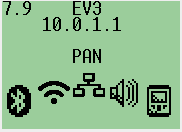
\includegraphics[width=.8\textwidth]{img/ev3_pan.png}
			\end{minipage}
			
			\item Nun navigierst du durch das Menü des Roboters wie auf den Bildern zu sehen und bestätigst jeweils mit der Auswahltaste: \textbf{USB-Client - Address - Advanced}
			
			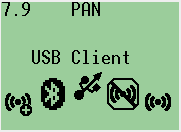
\includegraphics[width=.3\textwidth]{img/ev3_pan_usb.png}
			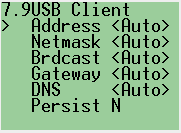
\includegraphics[width=.3\textwidth]{img/ev3_pan_usb_address.png}		
			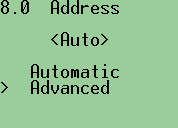
\includegraphics[width=.3\textwidth]{img/ev3_pan_usb_advanced.png}
			
			Nun musst du die IP Adresse 192.168.42.253 einstellen. Dazu navigierst du mit den rechts-/links-Tasten zu den einzelnen Ziffern und änderst deren Wert mit den oben-/unten-Tasten. Orientiere dich an den Bildern! Am Ende bestätigst du wieder mit der Enter-Taste. 
			
			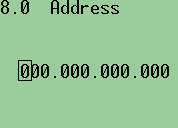
\includegraphics[width=.3\textwidth]{img/ev3_pan_usb_setip1.png}
			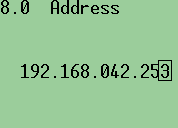
\includegraphics[width=.3\textwidth]{img/ev3_pan_usb_setip2.png}
			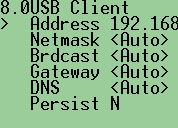
\includegraphics[width=.3\textwidth]{img/ev3_pan_usb_isset.png}
			
			\begin{minipage}{.6\textwidth}
				\item Mit der \textbf{Zurück}-Taste kommst du wieder in das Hauptmenü und die Einstellungen werden übernommen.
			\end{minipage}
			\hfill
			\begin{minipage}{.3\textwidth}
				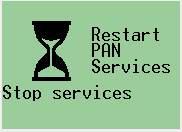
\includegraphics[width=\textwidth]{img/ev3_pan_usb_restart.png}
			\end{minipage}
			%		\\Nun kannst du wieder zu Punkt 3 auf Seite \pageref{sec:afterpan} wechseln.
		\end{enumerate}
		
		\section{Troubleshooting}
		\subsection{Installation über WLAN funktioniert nicht}
		Im Message-Server über \bfcode{File->Connected Devices }schauen ob alle Smartphones in der Liste auftauchen und der ADB-state auf \bfcode{connected} steht. 
		Ist dies nicht der Fall, tippe in der App auf \bfcode{TRENNEN} und stelle die Verbindung danach erneut her.
		Falls das nicht klappt, kontaktiere einen Betreuer. 
		Falls das Installieren per WLAN gar nicht mehr funktioniert, kann jederzeit eine USB-Verbindung zwischen Smartphone und PC hergestellt werden und darüber die App installiert werden.
		
		
		
		\section{Sensorbelegung}
		
		Tabelle	\ref{tab:sensors} zeigt die standardmäßige Sensorbelegung, wie sie in der App unter ``Mein Roboter'' definiert sein muss.\\
			
	
		\begin{table}[h]
			\begin{center}
				\begin{tabular}{r|l|l}						
					\textbf{Anschluss} & \textbf{Sensortyp} & \textbf{Modus} \\ \hline
					1 & Farbe & ColorID \\ 
					2 & Ultraschall & Distance \\ 
					3 & Gyroskop & Angle \\ 
					4 & Farbe & ColorID \\ 
				\end{tabular}
				\caption{Sensorbelegung}
				\label{tab:sensors}
			\end{center}
		\end{table}
	
		Tabelle \ref{tab:motors} zeigt den standardmäßigen Motoranschluss, wie er in der App unter ``Mein Roboter'' definiert sein muss.\\
		
		\begin{table}[h]
			\begin{center}
				\begin{tabular}{r|l}						
					\textbf{Anschluss} & \textbf{Motor} \\ \hline
					A & Large Regulated Motor \\ 
					B & - \\ 
					C & - \\ 
					D & Large Regulated Motor \\ 
				\end{tabular}
			\end{center}
			\caption{Motorbelegung}
			\label{tab:motors}
			\end{table}
	\end{document}		
	}{}
	
	\ifthenelse{\boolean{intro}}{
			\section{Hello World}
	In der Informatik ist es üblich, ein Hallo-Welt-Programm\footnote{https://de.wikipedia.org/wiki/Hallo-Welt-Programm} zu schreiben, wenn man eine Programmierumgebung kennenlernt. Deshalb fangen wir damit an. 
	Nachdem du den Roboter erfolgreich eingerichtet und das erste Mal getestet hast, gehen wir jetzt daran, uns den Quelltext näher anzusehen.
	\lstinputlisting[firstline=3]{\solpath/HelloWorld.java}
	Das Verhalten des Roboters befindet sich in der \textbf{run-Methode }(Zeilen 13-16). Wenn ein Mindroid-Programm ausgeführt wird, werden die Befehle in dieser Methode nacheinander abgearbeitet.
		\begin{itemize}
		\item{\bfcode{clearDisplay()}} löscht den Display-Inhalt
		\item{\bfcode{drawString(text, textsize, xPosition, yPosition)}} schreibt einen gegebenen Text (\bfcode{text}) an die gegebenen Koordinaten (\bfcode{xPosition, yPosition}) und verwendet dabei die definierte Schriftgröße (\bfcode{textsize}).
		\item Der Konstruktor in den Zeilen 8 bis 10 gibt unserem Programm einen Namen (Zeile 8). Mit dem Aufruf von \bfcode{super("Hello World")} bestimmen wir, unter welcher Bezeichnung unser Programm später ausgewählt werden kann. Es ist sinnvoll an beiden Stellen aussagekräftige Bezeichnungen zu verwenden.
		\end{itemize}
		Daneben gibt es noch die sogenannten “\textbf{imports}”. Da die Programm-Bibliotheken der MindroidApp sehr groß sind, hat jede Klasse einen ausführlichen Namen, der dabei hilft, den Überblick zu bewahren. Der Teil vor dem Klassennamen heißt \textbf{Paket} (engl. package). Zum Beispiel ist die Klasse \textbf{ImperativeWorkshopAPI} im Paket \textbf{org.mindroid.api.}
			\subsection{Der Ultraschallsensor - Abstand Messen}
	Um dich mit dem Ultraschall-Distanzssensor vertraut zu machen, implementiere den folgenden Code nach. Er stellt einen einfachen Parksensor dar, der wie folgt funktioniert:
	\begin{enumerate}
	\item Liegt die Distanz zu einem Objekt vor dem Roboter \textbf{unter 15cm}, dann blinkt die Status-LED schnell rot und es wird “\textbf{Oh oh :-O}” ausgegeben.
	\item Liegt die Distanz \textbf{zwischen 15cm und 30cm}, dann blinkt die Status-LED gelb und es wird “\textbf{Hm :-/}” ausgegeben.
	\item Liegt die Distanz \textbf{über 30cm}, dann leuchtet die Status-LED grün und es wird “\textbf{OK :-)}” ausgegeben.
	\end{enumerate}
	
	\lstinputlisting[firstline=3]{\solpath/ParkingSensor.java}
	
	\begin{itemize}
	\item Um die LED ansteuern zu können, müssen wir die Pakete \\ \bfcode{org.mindroid.api.ev3.EV3StatusLightColor}\\ und\\ \bfcode{org.mindroid.api.ev3.EV3StatusLightInterval} importieren.
	\item Wie in Zeile 19 zu sehen ist, läuft das Programm in einer Endlosschleife, bis der “Stop”-Knopf in der App betätigt wird.
	\item Wir müssen uns jeweils den vorherigen Zustand in der Variablen \bfcode{previousState} (Zeile 17) merken, da wir ansonsten alle 100ms den Zustand der LED zurücksetzen würden, was das Blinken verhindert. Mithilfe von \bfcode{previousState} ändern wir den LED-Modus nur dann, wenn wir müssen.
	
	\end{itemize}
		\subsection{Die Farbsensoren - Farbe messen}
	In dieser Aufgabe lernst du die Farbsensoren des Roboters kennen. Der folgende Quelltext liest kontinuierlich den aktuell gemessenen Farbwert des linken und rechten Lichtsensors aus (\bfcode{getLeftColor()} bzw. \bfcode{getRightColor()} in Zeilen 16 und 17).
	\\
	
	\lstinputlisting[firstline=3]{\solpath/ColorTest.java}
	
	\begin{itemize}
	\item Die Methode \bfcode{describeColor} (Zeilen 29-39) zeigt, wie du den Rückgabewert in einen lesbaren Text umwandelst.
	\item In den Zeilen 20-21 siehst du, wie man auf dem Display mehrzeiligen Text ausgeben kann. Die Buchstaben haben jeweils eine Höhe von 16 Pixeln, sodass die zweite Zeile an der y-Position 17 und die dritte Zeile an der y-Position 33 beginnt.
	\item Um die Qualität der Farbmessung näher zu betrachten, haben wir für dich Farbtafeln mit allen sieben unterstützten Farben des EV3-Lichtsensors vorbereitet. Bei welchen Farben funktioniert die Erkennung gut, bei welchen eher weniger?
	\item Der Farbsensor kann auch zur Erkennung von Abgründen eingesetzt werden: Welche Farbwerte werden gemessen, wenn der Roboter auf der Tischplatte steht und wenn die Farbsensoren über den Tischrand ragen?
	\end{itemize}
		\subsection{Kommunikation zwischen Robotern} % - Verteiltes ``Hallo Welt!''}
	In der vorherigen Aufgaben hast du kennengelernt, wie ein Programm auf einem einzelnen Roboter ausgeführt wird. Als nächstes wollen wir die Roboter \textbf{miteinander sprechen lassen}.
	
	Auch hier starten wir mit einem einfachen (diesmal verteilten) “Hallo Welt!”-Programm. Die Kommunikation läuft über das bereits vorgestellten “Server”-Programm, welches ihr vorhin schon auf dem Entwicklungsrechner gestartet habt. 
	
	Damit die Roboter voneinander unterschieden werden können, benötigt jeder einen eigenen Namen. Um diese Einstellungen ändern zu können, müsst ihr die Verbindung zum Server erst einmal trennen. Navigiert nun wieder in das Einstellungs-Menü der App und gebt den Robotern Namen. Stellt sicher, dass die Roboter auch in Gruppen eingeteilt sind. 
	
	Wiederhole diesen Schritt nun auch für den zweiten Roboter. In unserem Beispiel gehen wir davon aus, die Roboter heißen Robert und Berta.
	
	Wir möchten nun, dass Berta eine Nachricht mit dem Inhalt \textbf{``Hallo Robert!''} an den Nachrichtenserver versendet. Robert soll diese Nachricht empfangen und die Nachricht auf seinem Display ausgeben. 
	Dazu sind zwei unterschiedliche Programme für Robert und Berta notwendig.
	\lstinputlisting[firstline=3]{\solpath/HelloWorldPingA.java}
	\begin{itemize}
	\item Bei Programmstart sendet Berta in Zeile 16 eine Nachricht an \textbf{Robert }mit den Inhalt \textbf{``Hallo Robert!''}
	\end{itemize}
	
	\lstinputlisting[firstline=3]{\solpath/HelloWorldPingB.java}
	
	\begin{itemize}
	\item Robert überprüft mit \bfcode{hasMessage()} (Zeilte 16) ob neue Nachrichten auf dem Message-Server vorhanden sind. 
	\item Sobald eine Nachricht vorliegt, wird der Inhalt der Nachricht in die Variable \bfcode{msg} gespeichert (Zeile 16).
	\item die Nachricht wird nun mit dem String \textbf{``Hallo Robert!''} verglichen\footnote{Beachte: Strings werden in Java nicht mit == verglichen, sondern mittels der \bfcode{equals()}-Methode}. Stimmen beide überein, schreibt Robert auf sein Display einen Text (Zeile 19).
	\end{itemize}
	}{}
	
	\ifthenelse{\boolean{tasks}}{	
		\section{Mähroboter}
	\ifthenelse{\boolean{tasks}}{
	%	\easygcenter{.8\textwidth}{img/task_maehroboter.jpg}
		Nutze deine Kenntnisse, um den Roboter in einem mit schwarzem (oder weißem) Klebeband abgesperrten Bereich herumfahren zu lassen (so ähnlich wie beispielsweise viele Mähroboter arbeiten).
		\begin{enumerate}
		\item Wie beim Wand Ping-Pong soll der Roboter erstmal geradeaus fahren.
		\item Wenn er eine Grenze erkennt, soll er zurücksetzen und sich eine neue Richtung aussuchen.
		\item Beginne bei 1.
		\end{enumerate}
		
		Tipp: Überprüfe, welche Color-IDs auf dem Boden und den Begrenzungen erkannt werden, um festzustellen, wann der Roboter an die Umzäunung gelangt ist.
	}{}
	\ifthenelse{\boolean{scoring}}{
		Bewertungskriterien:
		\begin{itemize}
		\item (1P) Der umgrenzte Bereich darf nicht verlassen werden! Keines der Räder darf die Umgrenzung berühren!
		\item (1P) Vergleich: Wer schafft es am schnellsten, alle vier Seiten eines viereckigen Bereichs zu “treffen”?
		\end{itemize}
	}{}
	\ifthenelse{\boolean{solution}}{
		\sol{LawnMower}
	}{}		
		\section{Wand-Ping-Pong}
	\ifthenelse{\boolean{tasks}}{
		Nutze deine Kenntnisse, um den Roboter wie einen Ping-Pong-Ball in gerader Linie zwischen zwei Wänden/Gegenständen/... hin und her fahren zu lassen.
		Anweisungen:
		\begin{enumerate}
			\item Der Roboter soll solange geradeaus fahren, bis er eine Wand erkennt. Er soll dabei so nah wie möglich an die Wand heranfahren, ohne mit ihr zu kollidieren.
			\item Dann soll er ein kleines Stück rückwärts fahren und sich um 180° drehen
			\item Beginne bei 1.
		\end{enumerate}
	}{}
	\ifthenelse{\boolean{scoring}}{
		Bewertungskriterien:
		\begin{itemize}
			\item (1P) Ist die 180°-Drehung exakt?
			\item (1P) Vergleich: Wie nahe kommst du an die Wand heran?
			\item (1P) Vergleich: Wie schnell schaffst du eine Runde (Fahren $\rightarrow$ Wand+Drehen $\rightarrow$ Fahren)?
		\end{itemize}

	}{}
	\ifthenelse{\boolean{solution}}{		
		\sol{SingleWallPingPong}
	}{}
		\section{Platooning}
	\ifthenelse{\boolean{tasks}}{
	%	\easygcenter{.8\textwidth}{img/task_platooning.jpg}
		In dieser Aufgabe geht es darum, zwei Roboter hintereinander her fahren zu lassen, ohne dass es einen Auffahrunfall gibt. Aktuell forschen zahlreiche Unis und Unternehmen unter dem Schlagwort Platooning an genau dieser Problemstellung bei echten LKWs und PKWs: Die Fahrzeuge fahren dabei so nahe, dass sie den Windschatten des Vorausfahrenden ausnutzen können.
		
		Roboter A und B werden hintereinander platziert, sodass sie in die gleiche Richtung blicken. Ziel ist es zunächst, dass Roboter B den Abstand zu Roboter A in einem bestimmen Toleranzbereich hält. Die Distanzangaben im Folgenden sind nur mögliche Werte - du bestimmst selbst, was geeignete Grenzwerte sind.
		\begin{enumerate}
		\item Roboter A fährt los. Sobald der Abstand zwischen Roboter A und Roboter B größer als 35cm wird, beginnt Roboter B aufzuschließen.
		\item Wird der Abstand kleiner als 25cm, hält Roboter B die Geschwindigkeit von Roboter A .
		\item Wird der Abstand kleiner als 15cm, lässt Roboter B sich zurückfallen (oder fährt sogar rückwärts).
		\end{enumerate}
	}{}
	\ifthenelse{\boolean{scoring}}{
		Bewertungskriterien
		\begin{itemize}
		\item (1P) Roboter A und B fahren mind. 1 Meter hintereinander her ohne Kollisionen (weder mit anderen Robotern noch mit der Wand).
		\item (1P) Abstand bleibt in einem von euch zuvor bestimmten Bereich (Schnur), wenn beide Roboter vorwärts fahren.
		\item (1P) Vergleich: Geringstmöglicher Abstand, bei dem keine Kollision stattfindet.
		\end{itemize}
	}{}
	\ifthenelse{\boolean{solution}}{
		\sol{Platooning}
		\sol{PlatooningLeader}
		\sol{PlatooningFollower}
	}{}
		\section{Koordiniertes Wand-Ping-Pong}
	\ifthenelse{\boolean{tasks}}{
		Diese Aufgabe lehnt sich an die vorherige an. Allerdings sollen sich nun zwei Roboter abstimmen. Beide Roboter starten nebeneinander und blicken in die gleiche Richtung.
		Anweisungen:
		\begin{enumerate}
		\item Roboter A fährt solange, bis er eine Wand entdeckt. Er setzt zurück, dreht sich um und bleibt stehen.
		\item Roboter A sendet Roboter B eine “Start”-Nachricht.
		\item Daraufhin setzt sich Roboter B in Bewegung, bis er auf die Wand trifft. Daraufhin setzt Roboter B zurück, wendet und bleibt stehen.
		\item Roboter B sendet Roboter A eine “Weiter”-Nachricht.
		\item Beginne bei 1.
		\end{enumerate}
	}{}
	\ifthenelse{\boolean{scoring}}{	
		Bewertungskriterien:
		
		\begin{itemize}
		\item (1P) Roboter kollidieren nicht.
		\item (1P) Vergleich: Wie schnell schaffen die Roboter eine “Runde” (A: Fahren $\rightarrow$ Wand + Drehen + Stop; B: Warten $\rightarrow$ Fahren $\rightarrow$ Wand + Drehen + Stop)? Hier sollen die Roboter nicht möglichst nahe, sondern nahe genug an die Wand heranfahren (Abstand der Vorderachse kleiner 20cm).
		\end{itemize}
	}{}
	\ifthenelse{\boolean{solution}}{
		\sol{CoordWallPingPong}
		\sol{CoordWallPingPongA}
		\sol{CoordWallPingPongB}
	}{}

		\section{Dancing Robots}
	\ifthenelse{\boolean{tasks}}{
		%\easygcenter{.8\textwidth}{img/task_chachacha.png}
		Beim Cha-Cha-Cha gibt es die Tanzfigur “Verfolgung”. Dabei verfolgt jeweils ein Tanzpartner den anderen, bis beide sich umdrehen und die Rollen wechseln. Diese Figur ist tatsächlich nicht sehr weit vom Platooning-Beispiel aus der vorherigen Aufgabe entfernt.
		Der Ablauf soll dieses Mal wie folgt aussehen:
		\begin{enumerate}
		\item  Roboter A übernimmt zunächst das Kommando und fährt voraus, während Roboter B einen möglichst gleichbleibenden Abstand hält.
		\item  Roboter A beschließt nach einer gewissen Zeit, dass nun die Drehung folgt. Er stoppt und sendet eine “Drehen”-Nachricht an Roboter B.
		\item  Roboter B stoppt, wendet und sendet Roboter A eine “Gedreht”-Nachricht.
		\item  Daraufhin dreht Roboter A ebenfalls um 180°.
		\item  Nun tauschen Roboter A und B die Rollen: Roboter B fährt voraus und gibt den Ton bis zur nächsten Drehung an.
		\end{enumerate}
	}{}
	\ifthenelse{\boolean{scoring}}{
		Bewertungskriterien
		\begin{itemize}
		\item (1P) Einmal Verfolgung hin (Roboter A ist der Führende) und einmal Verfolgung zurück (Roboter B ist der Führende) und dabei keine Kollision!
		\item (1P) Es sollte klar erkennbar sein (bspw. per LED-Statusleuchte), wer aktuell der “Führende” ist.
		\end{itemize}
	}{}
	\ifthenelse{\boolean{solution}}{
		\sol{Follow}
		\sol{FollowA}
		\sol{FollowB}
	}{}
	}{}





\cfoot{\textcolor{lightgray} \today}




\end{document}
